% !TeX root = ./beamer.tex
%%%%%%%%%%%%%%%%%%%%%%%%%%%%%%%%%%%%%%%%%%%%%%%%%%%%%%%%%%%%%%%%%%%%%%
%
% Beamer template with UiT colour scheme
%
%%%%%%%%%%%%%%%%%%%%%%%%%%%%%%%%%%%%%%%%%%%%%%%%%%%%%%%%%%%%%%%%%%%%%%

\documentclass[xcolor=dvipsnames]{beamer} %
\usetheme[progressbar=frametitle,
  titleformat=smallcaps,
  % sectionpage=none,
  numbering=fraction,
  block=fill,
  background=dark]{metropolis}
% The below gives the font from a standard latex article, and should be used in pair.
\usetikzlibrary{arrows,shapes}
% If you want notes on the side:
% \setbeameroption{show notes on second screen=right} % Both
% \setbeamercolor{note page}{fg=yellow!10}
% \setbeamertemplate{note page}{
% 	\settowidth{\leftmargini}{\usebeamertemplate{itemize item}}
% 	\addtolength{\leftmargini}{-2\labelsep}
% 	\pagecolor{black!90}\vfill\insertnote\vfill
% }

\usepackage{utils/definitions}
\usepackage{utils/divide_toc}
\usepackage{utils/beamerouterthemesplit}
\usepackage{utils/citecmd}
\usepackage{utils/footfix}
\usepackage{utils/colors}
\setbeamerfont{footnote}{size=\tiny}

\title[Chemistry in CESM2]{Chemistry in CESM2}
\author{\textsc{Eirik Rolland Enger}}
\date{\vspace{-3mm}December 7, 2022\hfill
\includegraphics[width=4cm]{utils/CSU-Official-wrdmrk-Rev-2.png}}
\logo{\vspace{-2mm}
\includegraphics[width=15mm]{utils/CSU-Official-wrdmrk-Rev-2.png}\hspace{1mm}}
% \institute{UiT --- The Arctic University of Norway}
\begin{document}
\maketitle

% For every picture that defines or uses external nodes, you'll have to
% apply the 'remember picture' style. To avoid some typing, we'll apply
% the style to all pictures.
\tikzstyle{every picture}+=[remember picture]
% By default all math in TikZ nodes are set in inline mode. Change this to
% displaystyle so that we don't get small fractions.
\everymath{\displaystyle}

\section{Motivation}

\subsection{SSW}
\begin{frame}{Stratospheric Sudden Warmings}
  \begin{center}
    \copyrightbox[r]{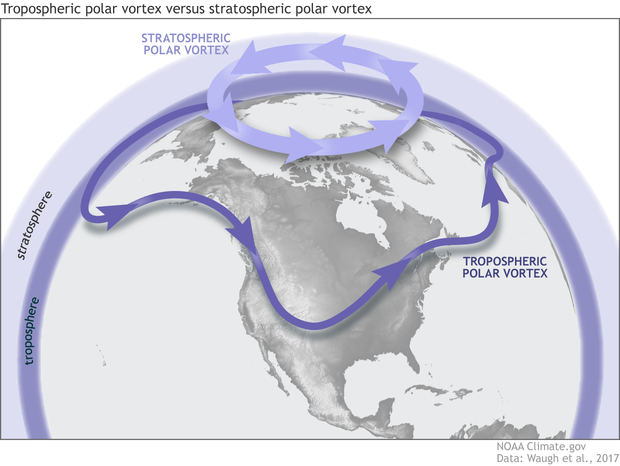
\includegraphics[width=0.85\linewidth]{./assets/Polar-Vortex.png}}
    {\tiny\href{https://www.climate.gov/news-features/blogs/enso/polar-vortex-going-make-you-put-sweater-be-afraid-be-very-afraid\#:~:text=Thus\%2C\%20the\%20tropospheric\%20polar\%20vortex,that\%20separates\%20the\%20air\%20masses.}{climate.gov}}
    % % -> \%
    % # -> \# OR ####
  \end{center}
  \note{
    \begin{itemize}
      \item SSWs, or stratospheric sudden warmings, are when the stratosphere is
            warmed by many kelvins. This is preceded by a wind reversal of the
            stratospheric polar vortex. I.e., the westerlies go eastward.
    \end{itemize}
  }
\end{frame}

\begin{frame}{Stratospheric Sudden Warmings}
  \begin{columns}
    \column{0.4\linewidth}
    \centering
    \copyrightbox[r]{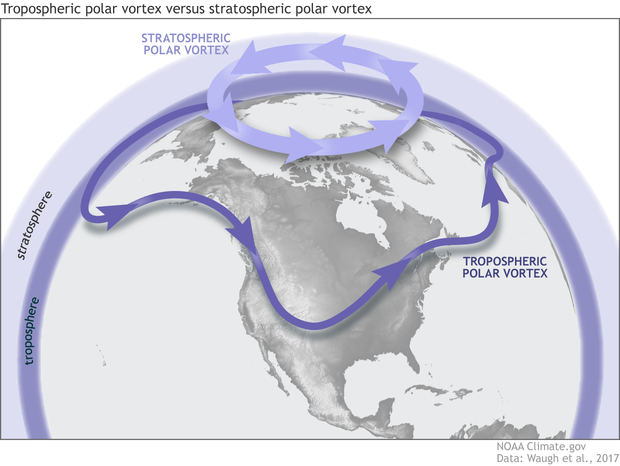
\includegraphics[width=\linewidth]{./assets/Polar-Vortex.png}}
    {\tiny\href{https://www.climate.gov/news-features/blogs/enso/polar-vortex-going-make-you-put-sweater-be-afraid-be-very-afraid\#:~:text=Thus\%2C\%20the\%20tropospheric\%20polar\%20vortex,that\%20separates\%20the\%20air\%20masses.}{climate.gov}}
    \column{0.7\linewidth}
    \begin{itemize}
      \item Defined as a wind reversal (eastward) at $ \SI{10}{\hecto\pascal} $ $ (\sim\SI{25}{\kilo\metre}) $, $ \SI{60}{\degree N} $
      \item Big improvement from including updated parametrizations of turbulent
            mountain stress (TMS), surface stress due to unresolved topography %marsh2013
      \item A lack of stratospheric internal variability without a high-top atmosphere %marsh2013
    \end{itemize}
  \end{columns}
  \note{
    \begin{itemize}
      \item The change in direction is what is used to define their occurrence
            and frequency.
      \item With the inclusion of turbulent mountain stress from unresolved
            topography, the SSW's saw a big improvement.
      \item Even though this is also part of the low-top version (CAM), the
            frequencies are too small, and WACCM get much closer to observation.
    \end{itemize}
  }
\end{frame}

\begin{frame}{Stratospheric Sudden Warmings}
  \begin{center}
    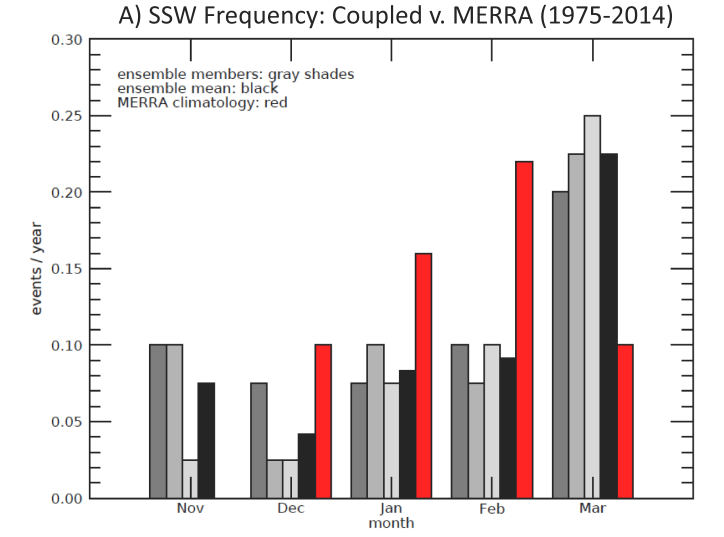
\includegraphics[width=0.8\linewidth]{./assets/ssw-freq.png}
  \end{center}
  \figurecite{gettleman2019}
  \note{
    \begin{itemize}
      \item Here we see frequency of SSW's between 1975 and 2014, in events per
            year. Three ensemble members in grayscale, the ensemble mean in black
            and observations in red.
    \end{itemize}
  }
\end{frame}

\subsection{Ozone}
\begin{frame}{Evolution of the Ozone layer}
  \footnotesize
  \begin{itemize}
    \item WACCM6 is able to reproduce the evolution of the ozone layer (also SH
          polar ozone hole)
    \item Ozone variability in the tropical stratosphere improves on the inclusion
          of an internally generated quasi-bilennial oscillation (QBO)  % marsh2013
  \end{itemize}
  \begin{center}
    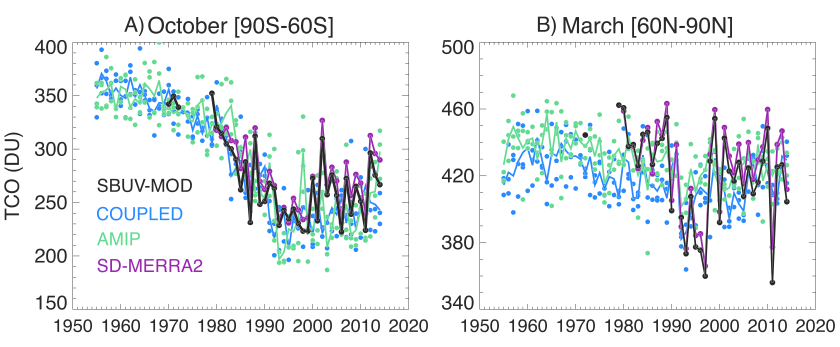
\includegraphics[width=0.85\linewidth]{./assets/ozone-2.png}
  \end{center}
  \figurecite{gettleman2019}
  \note{
    \begin{itemize}
      \item The figure is showing total column ozone in Dobson units from a WACCM6
            coupled simulation (blue) togheter with a specified SST (AMIP, green),
            specified dynamics (purple) and observations (black).
      \item If one look at ozone the biggest improvement is in the polar regions.
            WACCM6 is able to reproduce the evolution of the ozone layer, and also
            the SH polar ozone hole.
      \item One important improvement is the inclusion of an internally generated
            QBO. So again, stratospheric winds (but now in the tropical
            stratosphere) are needed to more precisely simulate a different
            physical process, ozone variability.
      \item Not shown are the tropics, where there are larger biases.
      \item \textit{
              (This is due to tropical upwelling; since the lower stratospheric
              ozone field is dynamically controlled, vertical velocity impact
              the total column ozone. And, larger vertical velocities in the
              lower stratosphere are expected to be associated with reduced
              ozone due to vertical advection of ozone poor air from the
              troposphere.)
            }
    \end{itemize}
  }
\end{frame}

\subsection{Atmospheric Blocking}
\begin{frame}{Atmospheric Blocking}
  \scriptsize
  Frequency of the meridional gradient of 500-hPa geopotential height below a
  threshold of $ \mathrm{GHGS}>0$, $\mathrm{GHGN}<\SI{-5}{\metre/degree} $
  \begin{align*}
    \mathrm{GHGS} & =\frac{Z(\phi_0)-Z(\phi_{\mathrm{S}})}{\phi_0-\phi_{\mathrm{S}}} \\
    \mathrm{GHGN} & =\frac{Z(\phi_{\mathrm{N}})-Z(\phi_0)}{\phi_\mathrm{N}-\phi_0}
    \label{eq:blocking-frequency}
  \end{align*}
  where \(\phi_{\mathrm{N}}=\SI{78.75}{\degree N}+\Delta\),
  \(\phi_{0}=\SI{60}{\degree N}+\Delta\), \(\phi_{\mathrm{S}}=\SI{41.25}{\degree N}+\Delta\)
  and \(\Delta=\SI{-3.75}{\degree},\SI{0}{\degree},\SI{3.75}{\degree}\) \cite{dandrea1998}.
  \note{
    \begin{itemize}
      \item Blocking frequency is another way tropospheric variability improve.
      \item A definition from D'Andrea et al. (1998) defines it as the frequency
            of the meridional gradient at 500-hPa geopotential height to be below
            a threshold of $ \SI{-5}{\metre/\degree} $.
      \item A given longitude is locally defined as blocked on a specific day if
            these conditions are satisfied for at least one of the three deltas.
    \end{itemize}
  }
\end{frame}

\begin{frame}{Blocking Frequency}
  \begin{figure}
    \begin{center}
      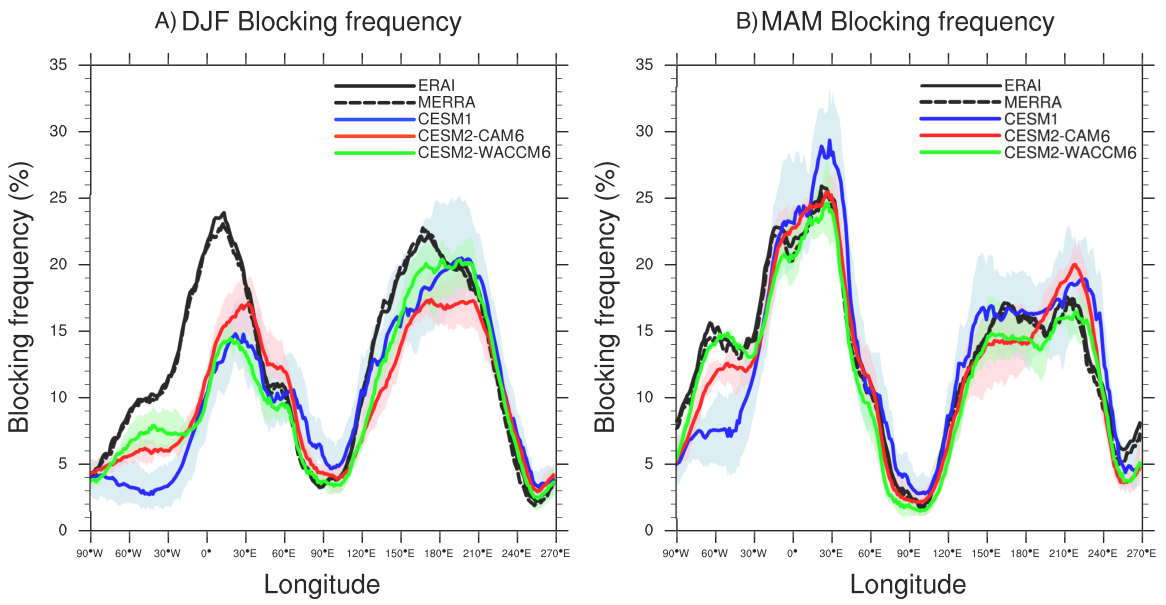
\includegraphics[width=0.95\textwidth]{./assets/blocking-2.png}
    \end{center}
    \label{fig:blocking-frequency}
  \end{figure}
  \figurecite{gettleman2019}
  \note{
    \begin{itemize}
      \item All simulations coupled to an active ocean. CESM1 has 35 simulations,
            CESM2-CAM6 5 simulations and CESM-WACCM6 3 simulations.
      \item CESM2 better than CESM1 in the Greenland blocking bump in March--May
            ($ \SI{30}{\degree W} $)
      \item CESM2 still has a DJF bias in the Atlantic sector.
      \item CESM2-WACCM6 significantly better than CESM2-CAM6 in the Pacific
            sector during DJF.
      \item With blocking frequency closer to observations, this indicates that
            stratospherical dynamical processes are important for high-latitude
            tropospheric climate variability.
    \end{itemize}
  }
\end{frame}

\subsection{Sea Ice}
\begin{frame}{Sea Ice}
  \footnotesize
  \begin{itemize}
    \item The September NH sea ice extent is better in WACCM6 than in CAM6
    \item Less downward surface SW and LW in WACCM6 due to higher LWP\footnote{liquid
            water path} which in turn is due to higher aerosol number.
  \end{itemize}
  $ \Rightarrow $ Tropospheric aerosol chemistry impacts Arctic sea ice.
  \begin{center}
    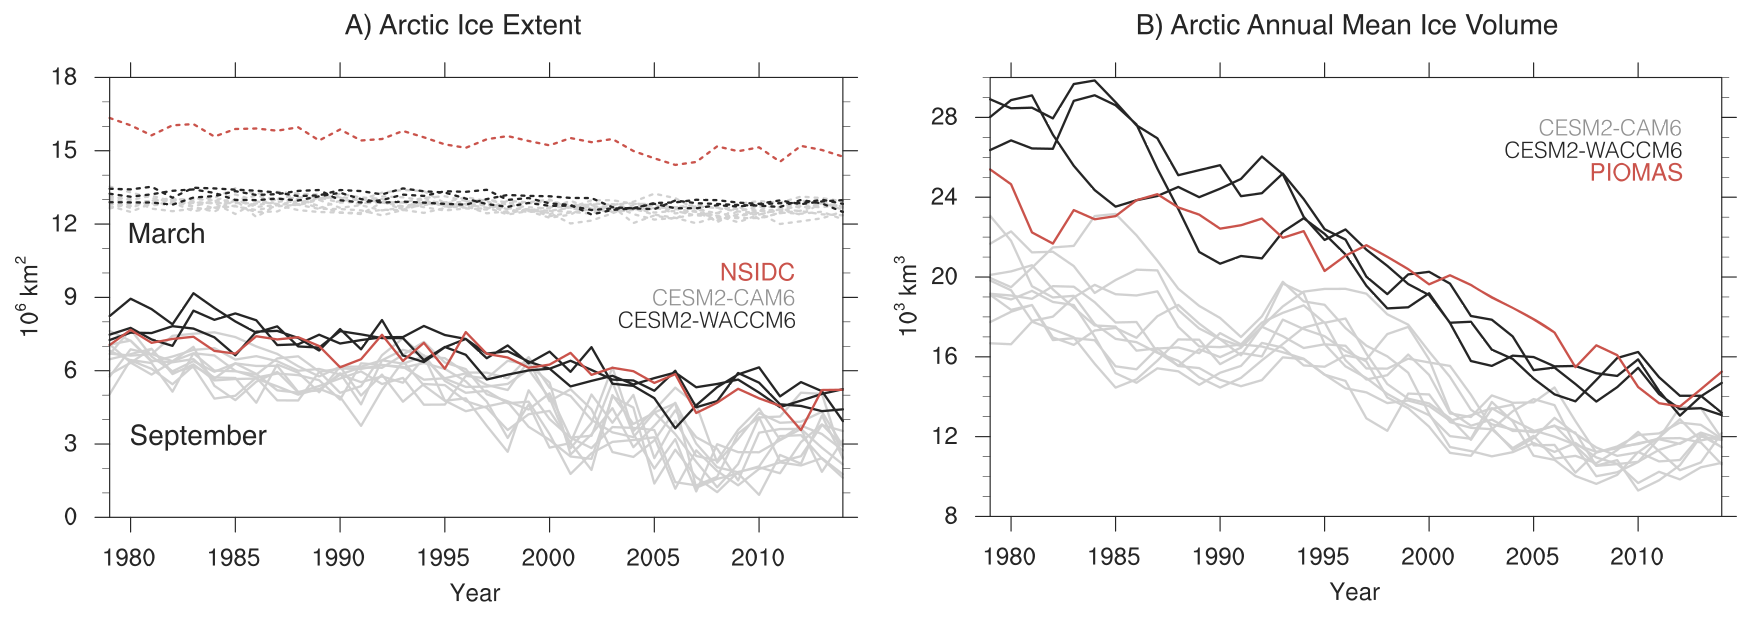
\includegraphics[width=0.95\linewidth]{./assets/ice-extent3.png}
  \end{center}
  \figurecite{gettleman2019}
  \note{
    \begin{itemize}
      \item With sea ice, you have an example of a process on the very bottom of
            the model that is noticeably affected by improving the resolution of
            the top of the atmosphere component.
      \item Annual mean sea ice extent is similar in CAM6 and WACCM6, both
            coupled, but WACCM6 has less melt in summer, resulting in thicker ice.
      \item The September NH sea ice extent is higher and in better accordance
            with observations in WACCM6 than in CAM6.
      \item The sea ice volume is dropping faster in WACCM6, faster than
            observations, while in CAM6 the rate is better while the volume is
            smaller.
      \item Have found that WACCM6 has less downward surface SW and LW because of
            slihtly higher liquid water path. In winter this is around the ice
            edge, in summer over the ice. This again is a result of higher aerosol
            number.
      \item We therefore find that tropospheric aerosol chemistry can make an
            impact on Arctic sea ice.
    \end{itemize}
  }
\end{frame}

\section{Implementation}

\subsection{Extra computations}
\begin{frame}{Computational Cost}
  \begin{table}
    \caption{Approximate costs of running different atmosphere models (From \href{https://www.cesm.ucar.edu/events/tutorials/2019/files/Lecture5a-mills.pdf}{lecture by Mills})}
    \label{tab:atm-model-cost}
    \scriptsize
    \begin{center}
      \begin{tabular}[c]{cccc}
        Configuration & Resolution                   & Chemistry & Core-hours/simulation years \\
        \hline
        CAM6          & $\SI{1}{\degree} $, $ 32 $ L & CAM       & $ \num{3700} $              \\
        WACCM6        & $\SI{2}{\degree} $, $ 70 $ L & MA        & $ \num{5400} $              \\
        WACCM6        & $\SI{1}{\degree} $, $ 70 $ L & TSMLT     & $ \num{22000} $             \\
        WACCM6-SC     & $\SI{1}{\degree} $, $ 70 $ L & SC        & $ \num{6000} $              \\
        WACCM6-SD     & $\SI{1}{\degree} $, $ 88 $ L & TSMLT     & $ \num{23000} $             \\
      \end{tabular}
    \end{center}
  \end{table}
  \note{
    \begin{itemize}
      \item We have now seen some of the improvements one might expect when using
            WACCM6 in favour of CAM6. But this comes at a cost. Let us see what
            that might be, before we look more closely at how and what extra is
            implemented in WACCM6.
      \item CAM is cheapest by quite a lot.
      \item Even the older MA version, which can only urn at nominal two degrees
            is close.
      \item SC: specified chemistry. Radiatively active chemical species (e.g.,
            ozone) are prescribed.
      \item SD: specified dynamics. Winds and temperatures are relaxed to a
            specific set of data (e.g.,  reanalysis from NASA GEOS).
    \end{itemize}
  }
\end{frame}

\subsection{Spatial}
\begin{frame}{Spatial}
  \begin{center}
    \copyrightbox[r]{
      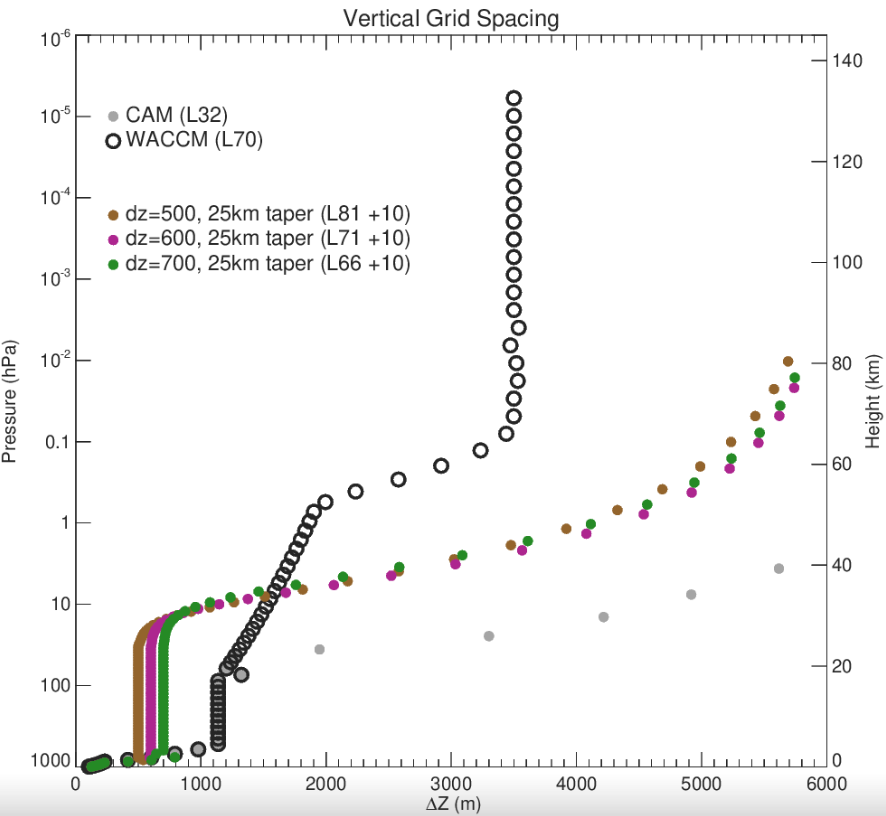
\includegraphics[width=0.7\linewidth]{./assets/vert-grid-2.png}
    }{\tiny\href{https://www.cesm.ucar.edu/working_groups/Atmosphere/dycore-res/vertical-phase-1.html}{cesm.ucar.edu}}
  \end{center}
  \note{
    \begin{itemize}
      \item The most obvious change is in vertical resolution.
      \item Brown, Purple and Green are just suggested new coordinates.
      \item Circles are WACCM6 and grey are CAM6, equivalent up to about
            $\SI{100}{\hecto\pascal}$.
    \end{itemize}
    See more at: \url{https://www.cesm.ucar.edu/events/wg-meetings/2018/presentations/amwgjoint/richter.pdf}
  }
\end{frame}

\subsection{Chemistry}
\begin{frame}{Chemistry Versions}
  \begin{itemize}[<+->]
    \item Neutral chemistry model versions of WACCM6
          \begin{itemize}
            \item TSMLT (troposphere, stratosphere, mesosphere, lower thermosphere) \textit{default}
            \item TS (troposphere and stratosphere mechanism)
            \item MA (Middle atmosphere)\begin{itemize}
                    \item Similar the older WACCM4, available in nominal $ \SI{2}{\degree} $ only %gettleman2019 table 1
                    \item Reduced set of tropospheric reactions
                  \end{itemize}
            \item MAD (Middle atmosphere with D region ion chemistry)
                  \begin{itemize}
                    \item Adds $ 15 $ positive and $ 21 $ negative ions % gettleman2019
                    \item Thus, below $ \SI{75}{\kilo\metre} $ electrons are no longer the main
                          negative charge carrier % gettleman2019
                  \end{itemize}
          \end{itemize}
    \item Additional thermosphere eXtension (WACCM-X)
  \end{itemize}
  \note{
    \begin{itemize}
      \item There are four chemistry packages to choose from when running WACCM6.
      \item TSMLT is the default in WACCM6, with troposphere, stratosphere,
            mesosphere and lower thermosphere included.
      \item TS is the troposphere and stratosphere mechanism.
      \item MA is the middle atmosphere version, included as a two degree option.
            It is very similar to the older default package used in WACCM4, and
            thus also has a reduced set of tropospheric reactions.
      \item But there is more! Mad! Middle atmosphere with D region ion chemistry
            included, that is.
      \item The D region is often used when talking about the ionosphere, as it is
            the lowest region in the ionosphere. It sits at around 60-80 km during
            the day and disappears during night.
      \item This version adds 15 positive and 21 negative ions, making it so that
            below $ \SI{75}{\kilo\metre} $, electrons are no longer the main
            negative charge carrier.
      \item Might also mention the eXtended versions while we're at it.
    \end{itemize}
  }
\end{frame}

\begin{frame}{Chemistry in TSMLT}
  \scriptsize
  MAM4 (\textit{Modal Aerosol Model}), also used in CAM6, but WACCM6 adds chemistry.
  \begin{itemize}
    \item Includes the chemical families \ce{O_x}, \ce{NO_x}, \ce{HO_x}, \ce{ClO_x} and \ce{BrO_x}, as well as \ce{CH4}
    \item Allows growth of sulfate aerosols, so the prognostic stratospheric aerosols can increase in width
    \item Maximum altitude of $ \SI{20}{\kilo\metre} $ for eruptions outputting more than $ \SI{3.5}{\tera\gram} $ \ce{SO2}
  \end{itemize}
  MOZART (\textit{Model for OZone And Related chemical Tracers})
  \begin{itemize}
    \item The chemical mechanism in CESM2, available from WACCM6, but also CAM-chem
    \item See \href{https://agupubs.onlinelibrary.wiley.com/action/downloadSupplement?doi=10.1029\%2F2019MS001882&file=jame21103-sup-0003-2019MS001882+Table_SI-S02.pdf}{table 2}\footnote{
            \url{https://agupubs.onlinelibrary.wiley.com/action/downloadSupplement?doi=10.1029\%2F2019MS001882&file=jame21103-sup-0003-2019MS001882+Table_SI-S02.pdf}}
          for a complete list of chemical reactions included in CESM2 when run with the TSMLT
          (troposphere, stratosphere, mesosphere, lower thermosphere) configuration.
  \end{itemize}
  \note{
    \begin{itemize}
      \item In charge of chemistry we find MAM and MOZART, not to be confused with
            MOSART (MOdel for Scale Adaptive River Transport).
      \item MAM includes the chemical families \ce{O_x}, \ce{NO_x}, \ce{HO_x},
            \ce{ClO_x} and \ce{BrO_x}, as well as \ce{CH4}.
      \item Also included are prognostic stratospheric aerosols. MAM4 was updated
            to allow for growth of sulfate aerosols into the coarse, or larger
            size, mode. This is important to represent aerosol sources (including
            volcanic emissions).
      \item The \ce{SO2} emissions from volcanic eruptions are derived from
            Volcanic Emissions for Earth System Models, which is based on
            observations. These observations then has to be accounted for, which
            is done by placing a maximum altitude on eruptions outputting more
            than $ \SI{3.5}{\tera\gram} $ \ce{SO2}. (The maximum altitude is to
            account for aerosol self-lofting due to in situ absorption of longwave
            radiation in estimating the initial altitude of large volcanic
            \ce{SO2} clouds.)
      \item MOZART takes care of the chemical mechanism, and can also be run in
            CAM-chem. A complete list of chemical reactions can be seen via link.
    \end{itemize}
  }
\end{frame}

\begin{frame}{Lumping}
  \begin{itemize}
    \item TSMLT has 231 solution species
    \item Species are lumped togheter to reduce the computational cost
    \item Example: \ce{C10H16} in MOZART-4 turned into five new lumped species, with
          \ce{APIN}, \ce{BPIN}, \ce{LIMON}, \ce{MYRC} and \ce{BCARY} giving the
          primary degradation rates.
  \end{itemize}
  \note{
    \begin{itemize}
      \item With that many reactions, 231 solution species, you have to draw the
            line at some point, but where?
      \item Lumping of chemical species is common.
      \item As an example, take \ce{C10H16} which was one lumped species in
            MOZART-4. This was turned into four monoterpenes and one
            sesquiterpene, with corresponding expansion of the oxidation scheme.
            The primary degradation rates were now based on alpha-pinene
            (\ce{APIN}), beta-pinene (\ce{BPIN}), limonene (\ce{LIMON}), myrcene
            (\ce{MYRC}) and beta-caryophyllene (\ce{BCARY}).
    \end{itemize}
  }
\end{frame}

\subsection{Solar and Geomagnetics}
\begin{frame}{Solar and Geomagnetics}
  \begin{itemize}
    \item Photoionization and heating rates uses parametrization of Solomon and Qian (2005), with input from the $ F_{10.7} $ index
    \item Ion-pair production rates are prescribed
    \item Low energy electrons included by the parametrized auroral oval model by
          Roble and Ridley (1994)
    \item Input to the model is HP, hemispheric power, related to the $ \mathrm{K_p} $
          index:
          \begin{equation*}
            HP=\left\{\begin{aligned}
               & 16.82\exp(0.32\mathrm{K_p})-4.86, & \mathrm{K_p}\leq 7 \\
               & 153.13+73.4(\mathrm{K_p}-7.0),    & \mathrm{K_p}>7
            \end{aligned}\right.
            \label{eq:hemispheric-power}
          \end{equation*}
    \item Since WACCM3, E region ionosphere is represented with a chemistry
          consisting of \ce{O+}, \ce{O2+}, \ce{N+}, \ce{N2+}, \ce{NO+}
  \end{itemize}
  \note{
    \begin{itemize}
      \item Photoionization and heating rates at wavelengths shorter than
            Lyman-$\alpha$, WACCM6 uses the parametrization of Solomon and Qian.
            This uses the $ F_{10.7} $ index as input.
      \item Ion-pair production rates by galactic cosmic rays, solar protons, and
            medium-energy electrons are prescribed
      \item For lower-energy electrons that precipitate in the auroral regions,
            WACCM6 use the parametrized auroral oval model by Roble and Ridley
            (1994) (implementation described in Marsh et al. (2007)). This model
            takes as input the power input to the atmopshere from energetic
            particle bombardment integrated over either the Northern or Southern
            Hemisphere, known as the Hemispheric Power in gigawatts.
      \item $ HP $ is assumed to be related to the $ \mathrm{K_P} $ index only,
            show here, formulation by Zhang and Paxton. If one wish to simulate
            for example solar storms, higher frequency forcing files can also be
            used.
    \end{itemize}
  }
\end{frame}

\appendix

\nocite{roble1994}
\nocite{solomon2005}
\nocite{garcia2007}
\nocite{marsh2007}
\nocite{marsh2013}
\nocite{mills2016}
\nocite{mills2017}
\nocite{gettleman2019}
\begin{frame}[allowframebreaks,plain]{References}

  \printbibliography[heading=none]

\end{frame}

\end{document}
